\documentclass[tikz,border=2pt]{standalone}
\usetikzlibrary{shapes.geometric}
\usetikzlibrary{decorations.pathreplacing}
\usetikzlibrary{calc}
\usetikzlibrary{positioning}
\usetikzlibrary{arrows.meta}
\usetikzlibrary{fit}
\usepackage{amsmath}
\usepackage{amssymb}
\usepackage{tikz}
\usepackage{xcolor}
\newcommand{\preserveresultheading}[1]{\BeforeBeginEnvironment{#1}{\Needspace{5\baselineskip}}}
\newcommand{\preserveresulttype}[1]{
  \AtBeginEnvironment{#1}{\crefalias{theorem}{#1}}}
\newcommand{\K}{K}
\newcommand{\Q}{\mathbb Q}
\newcommand{\Z}{\mathbb Z}
\newcommand{\N}{\mathbb N}
\DeclareMathOperator{\LS}{LS}
\DeclareMathOperator{\Cat}{Cat}
\DeclareMathOperator{\tp}{tp}
\DeclareMathOperator{\cl}{cl}
\DeclareMathOperator{\cf}{cf}
\DeclareMathOperator{\ci}{ci}
\DeclareMathOperator*{\colim}{colim}
\DeclareMathOperator{\id}{id}
\DeclareMathOperator{\Aut}{Aut}
\DeclareMathOperator{\dom}{dom}
\DeclareMathOperator{\ran}{ran}
\DeclareMathOperator{\rk}{rk}
\DeclareMathOperator{\otp}{otp}
\DeclareMathOperator{\supp}{supp}
\DeclareMathOperator{\Lim}{Lim}
\DeclareMathOperator{\Ord}{Ord}
\begin{document}
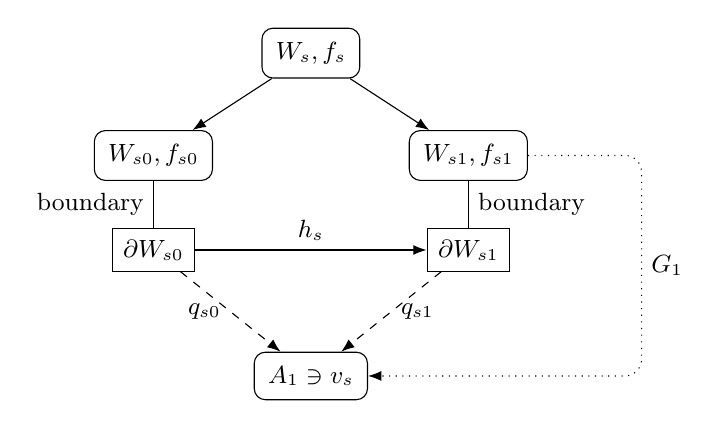
\begin{tikzpicture}[>=Latex, every node/.style={font=\small},
  world/.style={draw,rounded corners,inner sep=5pt},
  boundary/.style={draw,inner sep=4pt}]
 \node[world] (w) at (0,2.4) {$W_s,f_s$};
 \node[world] (w0) at (-2,1.1) {$W_{s0},f_{s0}$};
 \node[world] (w1) at (2,1.1) {$W_{s1},f_{s1}$};
 \node[boundary] (b0) at (-2,-.1) {$\partial W_{s0}$};
 \node[boundary] (b1) at (2,-.1) {$\partial W_{s1}$};
 \node[world] (a) at (0,-1.7) {$A_1\ni v_s$};
 \draw[->] (w) -- (w0);
 \draw[->] (w) -- (w1);
 \draw (w0) -- node[left] {boundary} (b0);
 \draw (w1) -- node[right] {boundary} (b1);
 \draw[->] (b0) -- node[above] {$h_s$} (b1);
 \draw[->,dashed] (b0) -- node[left] {$q_{s0}$} (a);
 \draw[->,dashed] (b1) -- node[right] {$q_{s1}$} (a);
 \draw[->,dotted,rounded corners=6pt] (w1.east) -- (4.2,1.1)
   -- node[right] {$G_1$} (4.2,-1.7) -- (a.east);
\end{tikzpicture}
\end{document}
